% This is samplepaper.tex, a sample chapter demonstrating the
% LLNCS macro package for Springer Computer Science proceedings;
% Version 2.20 of 2017/10/04
%
\documentclass[runningheads]{llncs}
%
\usepackage{graphicx}
% Used for displaying a sample figure. If possible, figure files should
% be included in EPS format.
%
% If you use the hyperref package, please uncomment the following line
% to display URLs in blue roman font according to Springer's eBook style:
% \renewcommand\UrlFont{\color{blue}\rmfamily}

\begin{document}
%
\title{Social Networks Analysis of Political Power and Elite Networks in Pakistan}
%
%\titlerunning{Abbreviated paper title}
% If the paper title is too long for the running head, you can set
% an abbreviated paper title here
%
\author{Syed Ammar Mahdi \and
Gohar Ayoub \and
Ahsan Qadeer}
%
\authorrunning{F. Author et al.}
% First names are abbreviated in the running head.
% If there are more than two authors, 'et al.' is used.
%
\institute{Habib University, Block 18, Gullistan e Johar, Karachi, Sindh, Pakistan
}
%
\maketitle              % typeset the header of the contribution
%
\begin{abstract}
This report briefly elucidates upon the human network of Pakistan's Members of National Assembly (MNAs). Both a structural approach and an actor centric approach is applied to two separate social networks. A structural approach is applied to study the social networks of MNAs based on their region, and an actor centric approach is applied to study the role of the infamous \textit{lotas}\footnote in Pakistani political networks. {A crude term to refer to someone who politically switches parties for their own gain.} By taking a closer look at the actors who switched parties to successfuly win a seat from PTI, the role of such actors in affecting the overall political elite network is examined.

\keywords{Member National Assembly  \and Homiphily \and Group internal/external ties}
\end{abstract}
%
%
%
\section{Introduction}

The topic of this report is "Social Networks Analysis of Political Power and Elite Networks in Pakistan". The scope of the method studied is social network analysis using the relevant graph theory metrics studied, as well as a new metric: the Krackhardt E-I index. This social network analysis is applied to the list of Members of National Assembly to calculate Homophily. By examining the overall structure of the national assembly at both a regional level and within the ruling government party (PTI), the role of both individual actors who have switched political factions (i.e. \textit{Lotas}) and the overall structure of the networks of the political elite, as reflected within the ties of the National Assembly, will be discussed in this report.

\section{Background and Scope}

\section{Examples of Application}
The political history of Pakistan is characterized by ruptures in the institution of democracy through coups staged by military forces due to different reason with similar basic motivation of acquiring power of political decision-making. After half a century of discontinuances in the institute of democracy, it has only been very recently that Pakistan has moved towards complete democratization. The successful completion of three different democratically elected by three different national parties and smooth transitions of power in between warrants a study into this movement towards democratization and the role of different actors in the spatial context of democratic Islamic Republic of Pakistan.
\indent
The democratization of any state can be explained through structural theories or actor-centric theories. Structural explanatory paradigm proclaims that socio-economical, industrial and educational factors play a primary role in stabilization of already existing democracies or, in the absence of democracy. a movement towards democratisation (Seymour, 1959). Contrary to this, actor-centric theory try to explain the emergence of democracy or democratic stability to elite bargaining and strategic interactions between them (Guillermo and Philippe, 1986). Historically, it can be argued that structural factors can play a major role in explaining the processes of democratization for several countries across the globe. However, according to Doorenspleet and Kopecky (2010), there are some anomaly states where actor-centric explanations hold more power than their counterparts because of inter-connectivity of elites in the any prevailing political systems of governance.
\indent
This paper tries to investigate the authenticity of actor-centric explanation for the recent democratic stabilization in Pakistan through study of networks of Members of National Assembly elected in 2018 using the parameters of previous and current party affiliations. Although the quality of democracy in Pakistan is questionable due to interference of extra-democratic military actors in the democratic processes, the move from autocratic regime of military leaders to a less transparent system rewarding public opinion is significant enough to bring about an economic, social and political shift for the common populace. This paper will also try to investigate the effect of this structural political change on the power relations within elites and of elites with different political and non-political parties.
\indent
Osei (2015) and Efim (2013) investigate the structure of political elites in Ghana and Polish state respectively. This paper uses the theoretical concepts used in the paper "Elites and democracy in Ghana: A social network approach" to understand the political networks of elites in Pakistan and their party fluidity depending on the prevailing democratic political power structure in the country. The idea of analysis of the network over a period of time definitive of political landscape is borrowed from the paper "The structure of political elite network in the Republic of Poland in 1993 - 2013" where the author of the paper identifies two periods of political formation in Poland. Similarly, this paper recognizes the importance of temporal context in formulation and stabilization of democratic infrastructures in Pakistan by identifying the period of 2008 to 2018 as crucial.
\indent
Seymour Martin Lipset, ‘Some social requisites of democracy: Economic development
and political legitimacy’, American Political Science Review, 53 (1959), pp. 69–105.\\
Guillermo A. O’Donnell and Philippe C. Schmitter, Transitions from authoritarian rule
(Johns Hopkins University Press, Baltimore, MD, 1986)\\
Doorenspleet and Kopecký, ‘Against the odds’, p. 710; see also Jan Teorell, Determinants
of democratization: Explaining regime change in the world, 1972–2006 (Cambridge University
Press, Cambridge, 2010).\\
Osei, A. (2015). Elites and democracy in Ghana: A social network approach. African Affairs, 114(457), 529-554.\\
Efim, F. (2013). The structure of political elite networks in the Republic of Poland in 1993-2013. Baltic Region, 5(4).\\
\section{Examples to a Contextualized Case study}

\begin{figure}
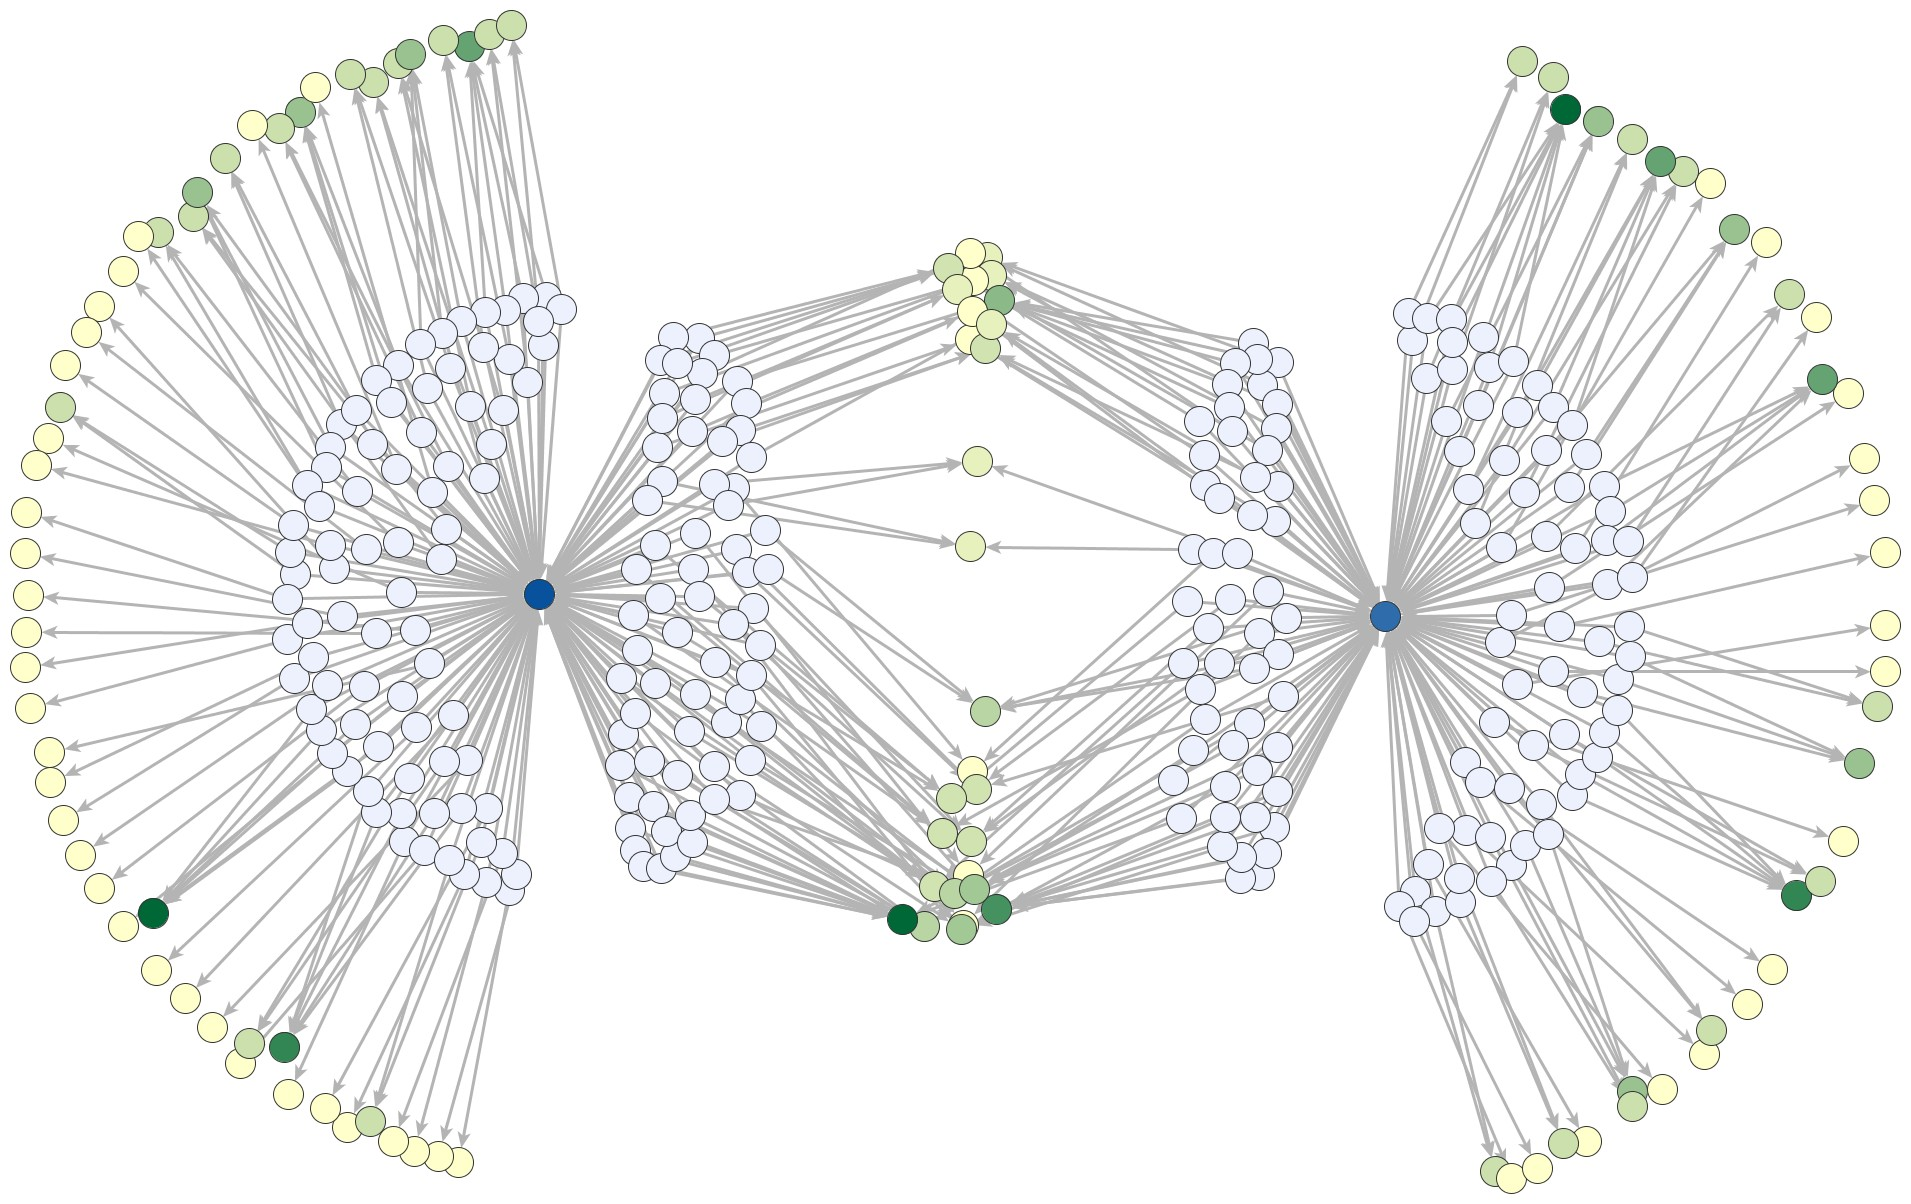
\includegraphics[width=\textwidth]{bowtie_structure.jpg}
\caption{The model of the national assembly of Pakistan as a social network. The graph has a resemblance to a bow-tie structure. The } \label{fig1}
\end{figure}

\begin{figure}
\includegraphics[width=\textwidth]{formerparties.jpg}
\caption{A figure caption is always placed below the illustration.
Please note that short captions are centered, while long ones are
justified by the macro package automatically.} \label{fig1}
\end{figure}

\begin{figure}
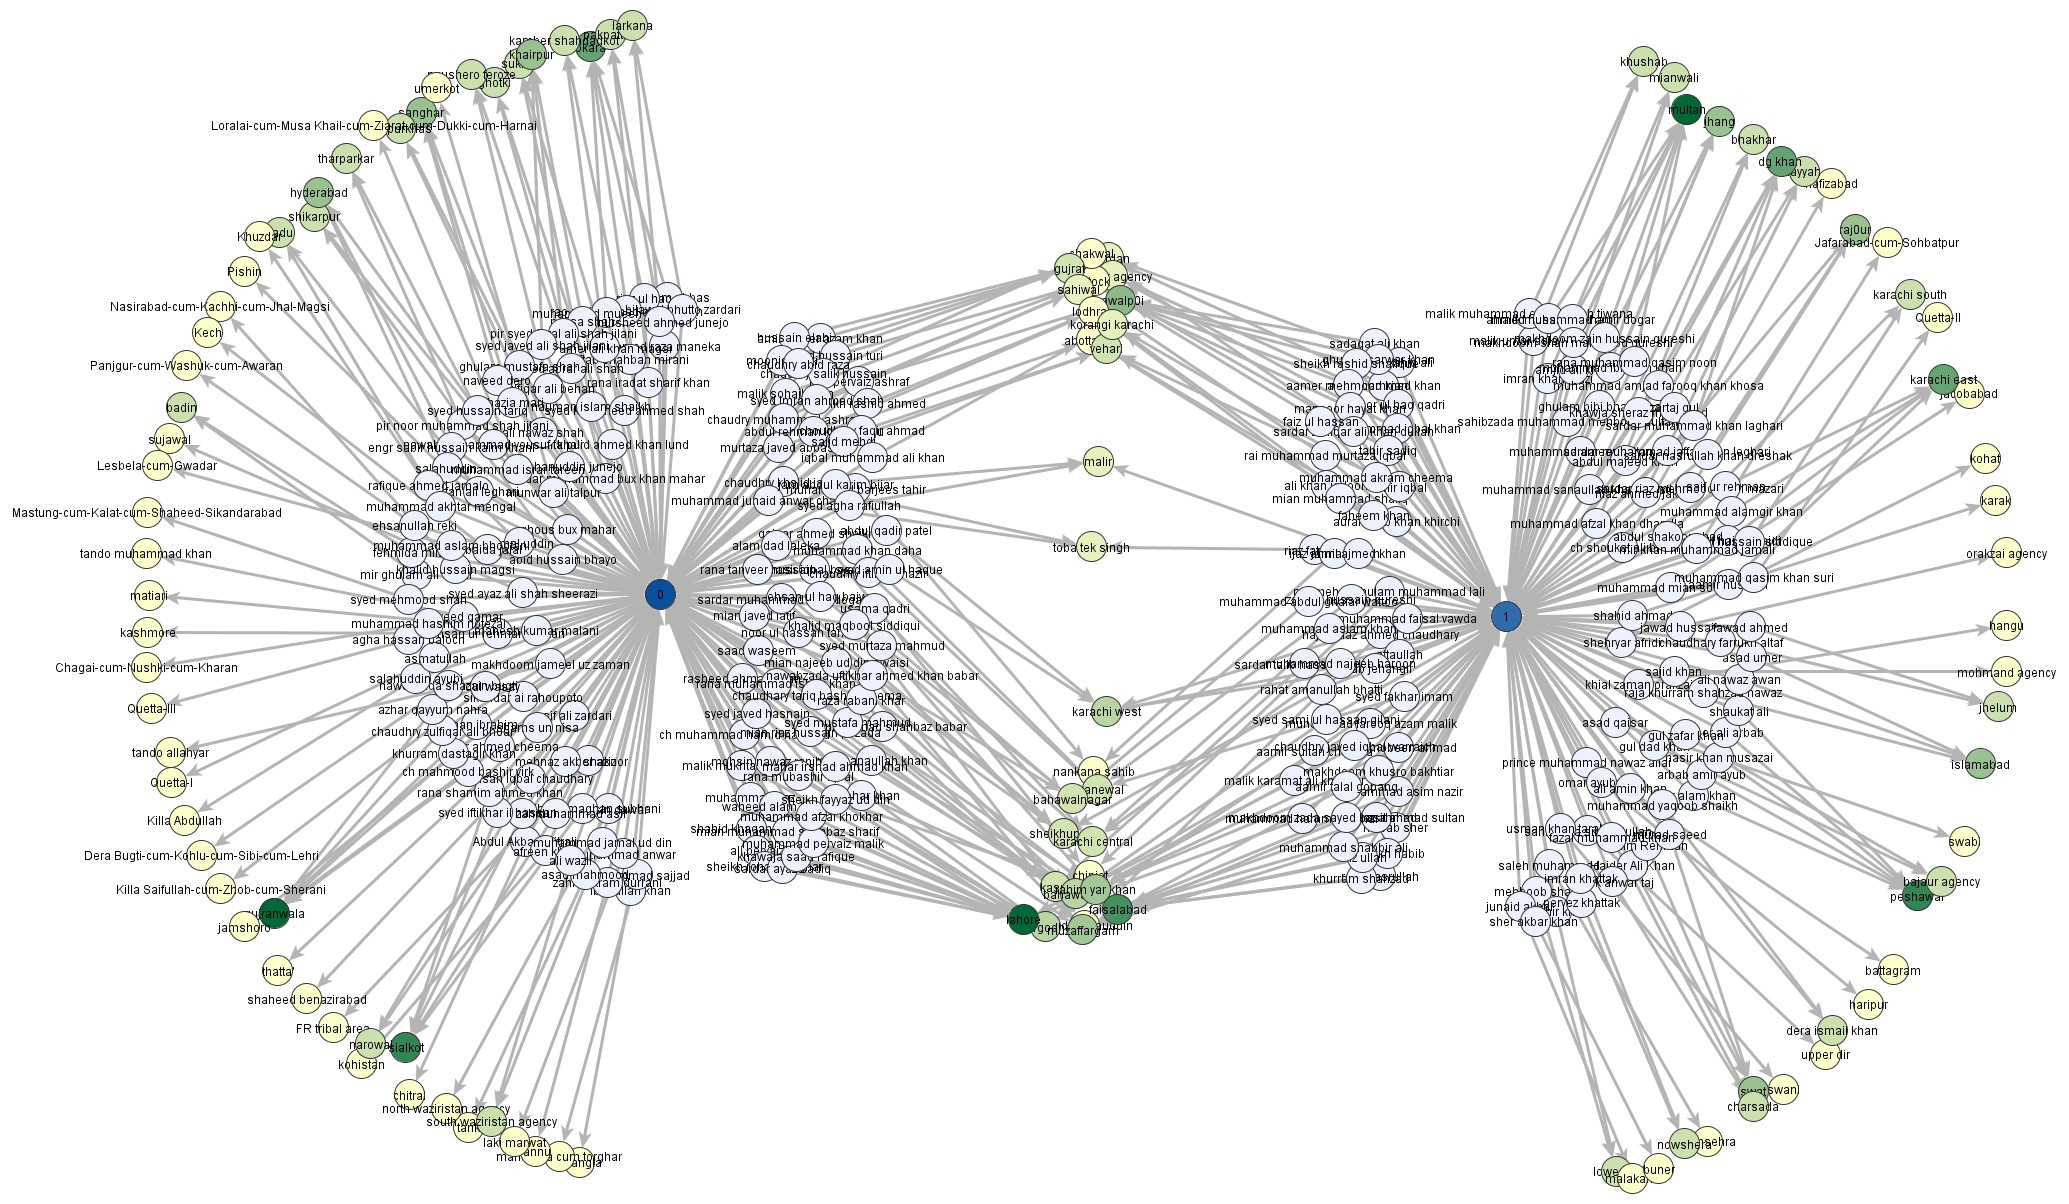
\includegraphics[width=\textwidth]{labelled_mna_sheet.jpg}
\caption{A figure caption is always placed below the illustration.
Please note that short captions are centered, while long ones are
justified by the macro package automatically.} \label{fig1}
\end{figure}

\begin{figure}
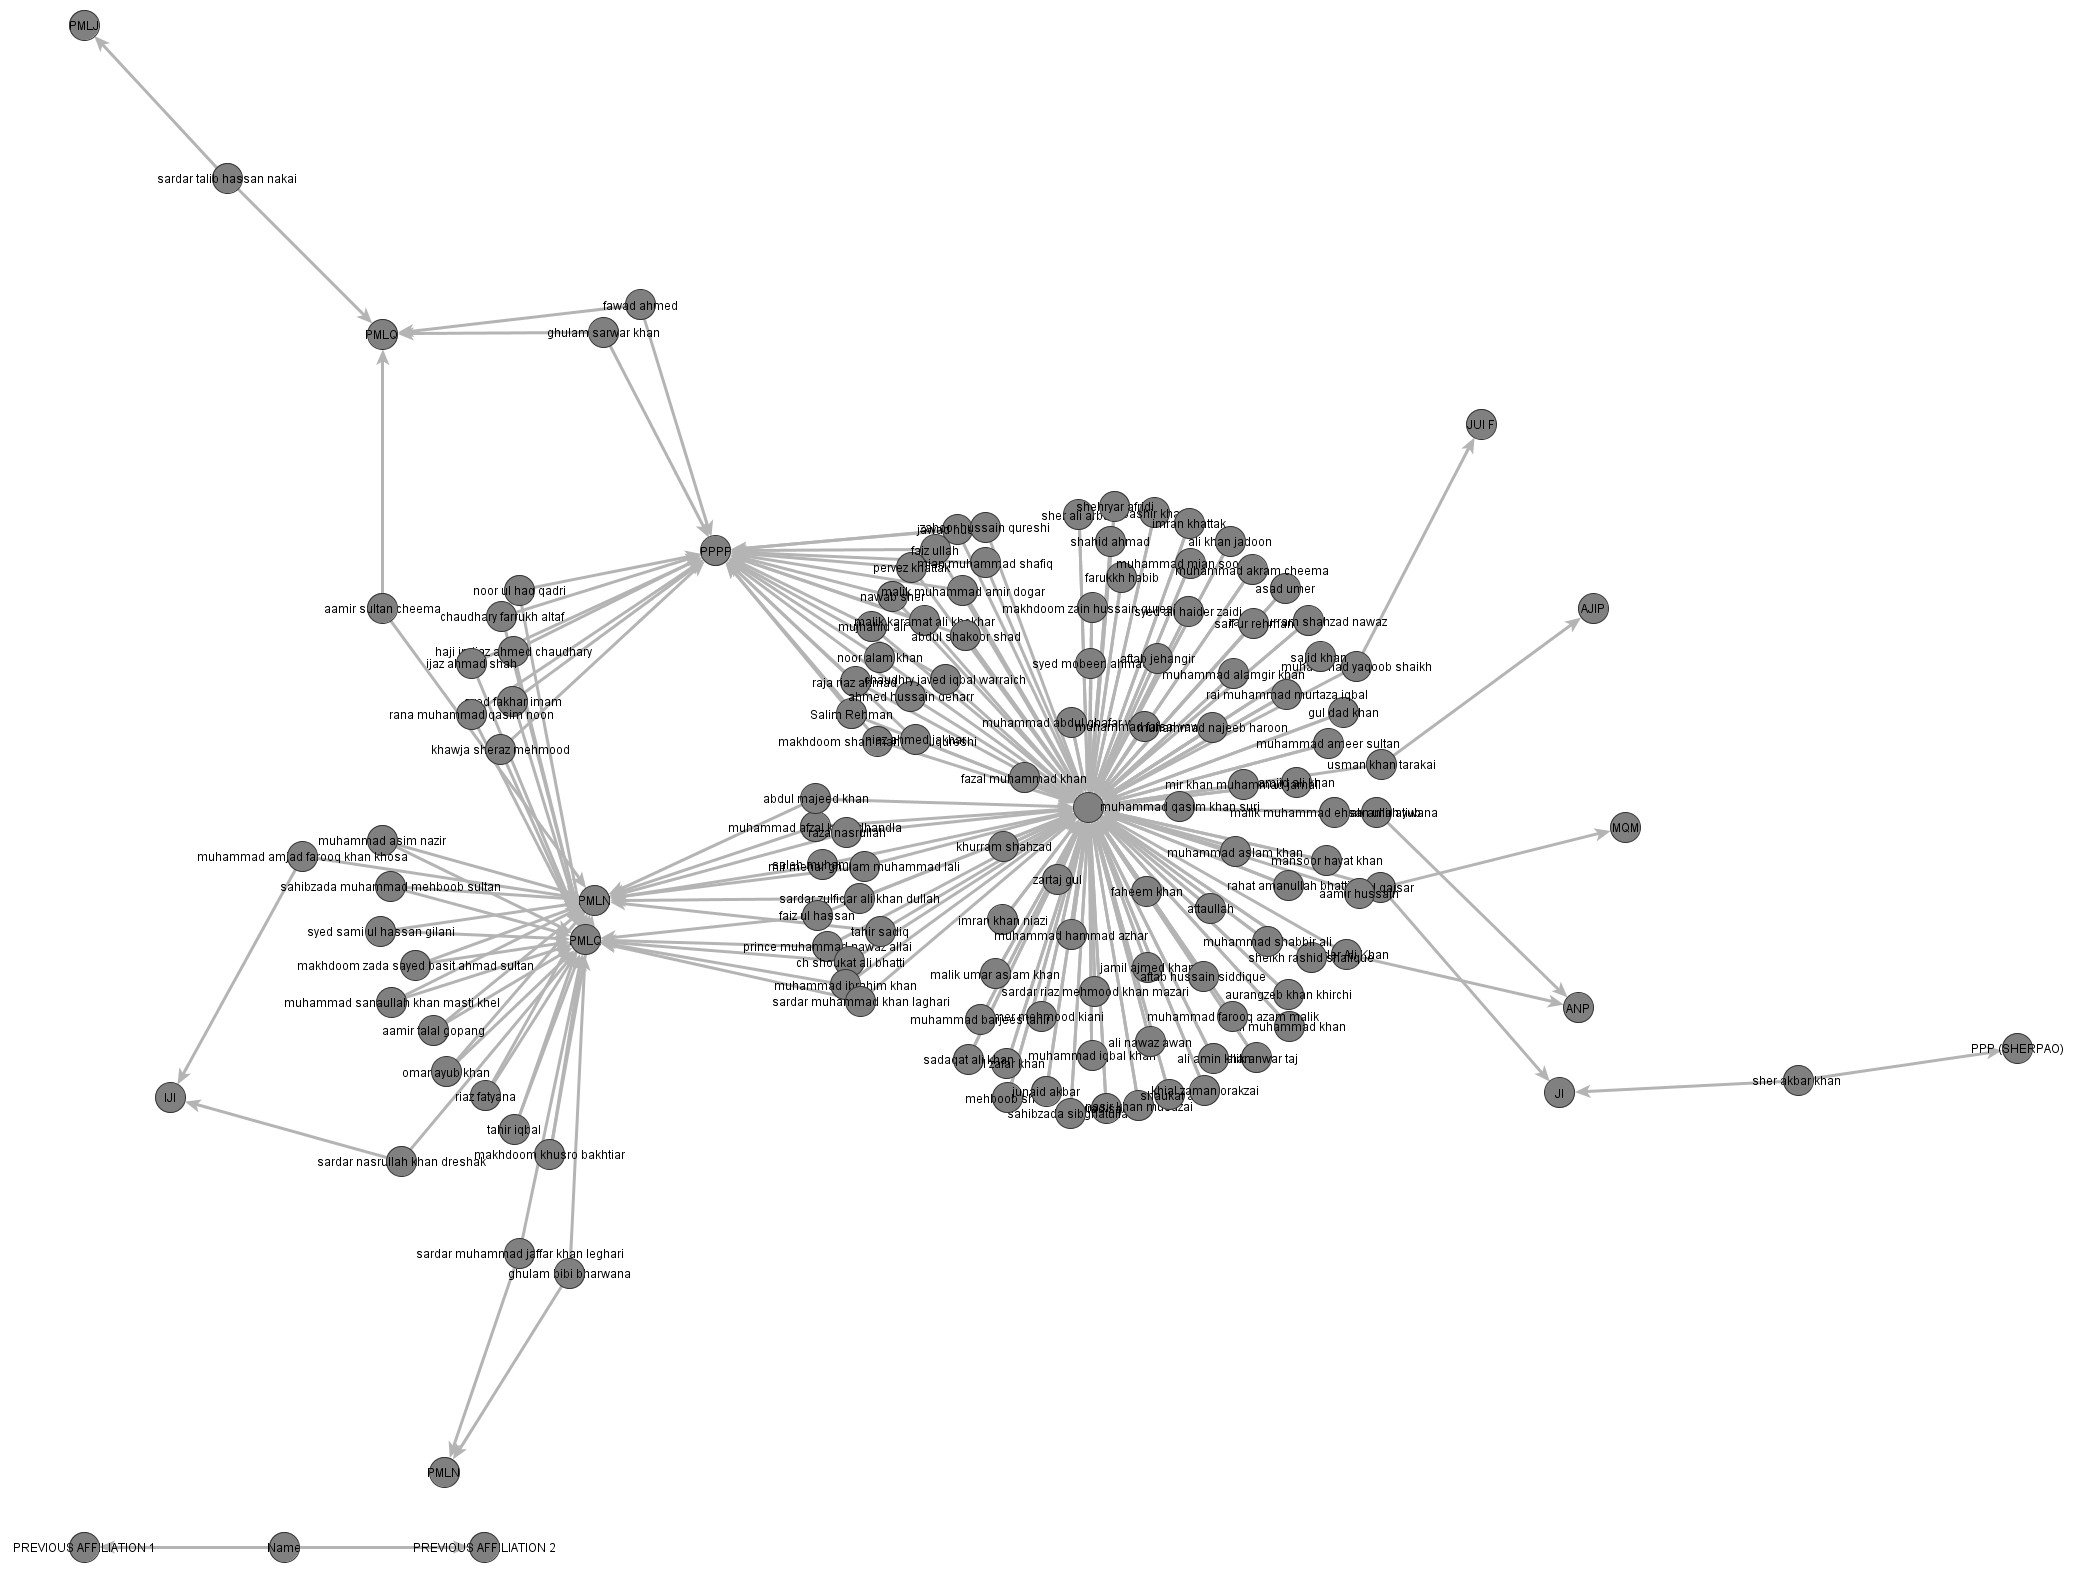
\includegraphics[width=\textwidth]{formerparties1.jpg}
\caption{A figure caption is always placed below the illustration.
Please note that short captions are centered, while long ones are
justified by the macro package automatically.} \label{fig1}
\end{figure}


For citations of references, we prefer the use of square brackets
and consecutive numbers. Citations using labels or the author/year
convention are also acceptable. The following bibliography provides
a sample reference list with entries for journal

\begin{thebibliography}{8}
articles~\cite{ref_article1}, an LNCS chapter~\cite{ref_lncs1}, a
book~\cite{ref_book1}, proceedings without editors~\cite{ref_proc1},
and a homepage~\cite{ref_url1}. Multiple citations are grouped
\cite{ref_article1,ref_lncs1,ref_book1},
\cite{ref_article1,ref_book1,ref_proc1,ref_url1}.
\end{thebibliography}
\end{document}
